\documentclass[11pt,german]{article}
\usepackage[T1]{fontenc}
\usepackage[latin9]{inputenc}
\usepackage[left=2cm,right=2cm,top=2.5cm,bottom=2.5cm]{geometry}
\usepackage{tikz}
\usetikzlibrary{er,arrows,positioning}
\usepackage{ragged2e}
\usepackage[normalem]{ulem}
\usepackage[fleqn]{amsmath}
\usepackage{amssymb}
\usepackage{babel}
\RequirePackage{vsis-gdb}

\title{GDb Aufgabenblatt 3}
\author{Tim Kromer, Luke Kroll, Sven Schmidt}


\begin{document}

\tikzstyle{erbt} = [->, >=open triangle 90, thick]
\tikzset{ermod/.style={rectangle,thick,draw=black!45,
		fill=black!5,minimum size=4mm}}
\maketitle

\section*{1. Informationsmodellierung mit dem Entity-Relationship-Modell}


\begin{center}
\begin{tikzpicture}

\node[entity](instrument) at (0,6) {Instrument}
node [entity] (vereinsmitglied)  at (0,0) {Vereinsmitglied}
node [entity] (musiker) at (0,2) {Musiker}
edge [erbt] (vereinsmitglied)
node [entity] (chorleiter) at (9,6) {Chorleiter}
edge [erbt] (musiker)
node [entity] (veranstaltung) at (0,-6) {Veranstaltung}
node [entity] (performance) at (5,-9) {Performance}
node [entity] (musikstück) at (-5,-9) {Musikstueck}
node [relationship] (komp) at (-5,2) {komponiert}
edge (musiker)
edge (musikstück)
node [relationship] (org) at (-2,-3) {organisiert}
edge (vereinsmitglied)
edge (veranstaltung)
node [relationship] (bes) at (2,-3) {besucht}
edge  (vereinsmitglied)  
edge (veranstaltung)
node [relationship] (spielt) at (0,4) {spielt} 
edge (musiker)
edge (instrument)
node[relationship] (teil) at (5,2) {nimmt teil}
edge (musiker)
edge (performance)
node[relationship] (leitet) at (9,-9) {leitet}
edge (chorleiter)
edge (performance)
node[relationship] (aufführung) at (0,-9) {Auffuehrung}
edge (veranstaltung)
edge (performance)
edge (musikstück)
node (besMit) at (1.5,-1) {[0,*]}
node (orgMit) at (-1.5,-1) {[0,*]}
node (besVer) at (1.5,-5) {[0,*]}
node (orgVer) at (-1.5,-5) {[1,*]}
node (spIn) at (-0.5,5) {[0,*]}
node (spMu) at (-0.5,3) {[0,*]}
node (koMu) at (-2.5,2.5) {[0,*]}
node (koSt) at (-5.5,-3) {[1,1]}
node (leiCho) at (9.5,-1) {[0,*]}
node (leiPer) at (7.5,-9.5) {[1,1]}
node (teiMu) at (2.5,2.5) {[0,*]}
node (teiPer) at (5.5,-3) {[1,*]}
node (aufPer) at (2.5,-9.5) {[1,1]}
node (aufVer) at (0.5,-7) {[1,5]}
node (aufSt) at (-2.5,-9.5) {[0,*]}
node [attribute] (in-Bez) at (-3,6) {\underline{Bezeichnung}}
edge (instrument)
node [attribute] (in-Teile) at (2.5,6) {Teile}
edge (instrument)
node [attribute] (chJahre) at (6,6) {Chorjahre}
edge (chorleiter)
node [attribute] (mitNr) at (-3,1) {\underline{Mitgliedsnr.}}
edge (vereinsmitglied)
node [attribute] (mitNa) at (-3,-0.5) {Name}
edge (vereinsmitglied)
node [attribute] (mitDat) at (3,1) {E.datum}
edge (vereinsmitglied)
node [attribute] (stTitl) at (-3,-8) {\underline{Titel}}
edge (musikstück)
node [attribute] (verBez) at (-3,-6) {\underline{Bez.}}
edge (veranstaltung)
node [attribute] (verDat) at(3,-6) {Datum}
edge (veranstaltung)
node[attribute] (perTitl) at (3,-8) {\underline{Titel}}
edge (performance)
node [attribute] (perEnd) at (7.5,-8) {Endzeit}
edge (performance)
node [attribute] (perStart) at (6.5, -7) {Startzeit}
edge (performance)
;

\end{tikzpicture}
\end{center}

\section*{2. Relationales Datenmodell}
\subsection*{a)}
\begin{center}
	\begin{tikzpicture}[node distance=.5cm,every node/.style={draw,ermod}]
		\node[text width=6cm,align=left](erbt){\begin{RMSchma}		
		Set(\underline{SNr},Alter)
		\\
		Verkaufsset(\underline{SNr},LPreis)
		\\
		Werbeset(\underline{SNr}, Firma)	
		\end{RMSchma}};
	\node[below=of erbt,text width=8cm,align=left](besitzt){\begin{RMSchma}
		Thema(\underline{Bez})
		\\				
		 Set(\underline{SNr},Alter,\dashuline{Thema$\Rightarrow$Thema.Bez})	
		\end{RMSchma}};
	\node[below=of besitzt,text width=14cm,align=left](zugeordnet){\begin{RMSchma}
		Thema(\underline{Bez})	
		\\			
		Modell(\underline{(Name,Datum)},Grad)
		\\
		Zugeordnet(\dashuline{Bez$\Rightarrow$Thema.Bez,(Name,Datum)$\Rightarrow$(Modell.Name,Modell.Datum)})	
		\end{RMSchma}};
	\node[below=of zugeordnet, text width=8cm,align=left](hat){\begin{RMSchma}
		Farbe(\underline{RGB},CMYK)
		\\				
		Baustein(\underline{Form},Bild,\dashuline{Farbe$\Rightarrow$Farbe.RGB})	
		\end{RMSchma}};
	\node[below=of hat, text width=12cm,align=left](enthaelt){\begin{RMSchma}
		Set(\underline{SNr},Alter,\dashuline{Thema$\Rightarrow$Thema.Bez})
		\\
		Baustein(\underline{Form},Bild,\dashuline{Farbe$\Rightarrow$Farbe.RGB})
		\\
		Farbe(\underline{RGB},CMYK)
		\\				
		Modell(\underline{(Name,Datum)},Grad)
		\\
		enthaelt(\dashuline{SNr$\Rightarrow$Form$\Rightarrow$Baustein.Form,Farb$\Rightarrow$Farbe.RGB,}
		\\
		\hspace{1.5cm} \dashuline{(Name,Datum)$\Rightarrow$(Modell.Name,Modell.Datum)})	
		\end{RMSchma}};
	\end{tikzpicture}
\end{center}
\subsection*{b)}
Da beim Hausklassenmodell alle Erben ihre eigene Tabelle (Hausklasse) erhalten und keine Referenz in ihrer Superklasse, bräuchte jeder Erbe eine eigene Relation (sofern es eine Relation zwischen der jeweiligen Superklasse und irgendeiner anderen Entität gibt).  


\section*{3. Relationale Algebra und SQL}
\subsection*{a)}
\subsubsection*{i)}
\begin{align*}
&\pi_{Titel}(\sigma_{Seitenzahl>200\land Erscheinungsjahr>1950}(Buch))\\
&=\{'Hundert\> Jahre\> Einsamkeit','Requiem\> fuer\> einen\> Traum','Der\> Talisman'\}
\end{align*}

\subsubsection*{ii)}
\begin{align*}
&\pi_{Vorname,Nachname}(\sigma_{Buch="Der Talisman}(Schreibt)\underset{Autor=PID}{\Join}Person)\\
&=\{('Stephen','King'),('Peter','Straub')\}
\end{align*}
\subsubsection*{iii)}
\begin{align*}
&\pi_{Vorname,Nachname}(Person\underset{PID=Lektor\land Lieblingsbuch=Buch}{\Join}Begutachtet)\\
&=\{('Leo','Tolstoi'),('Fjodor','Dostojewski'),('Gabriel','Garcia\> Marquez')\}
\end{align*}
\subsection*{b)}
\subsubsection*{i)}
Alle Bücher die noch nicht begutachtet wurden.
\begin{align*}
&=\{('Schall\> und \> Wahn', 1929, 304, 'Diogenes'),('Der\> Talisman', 1984, 714 'Heyne')\}
\end{align*}
\subsubsection*{ii)}
Vorname und Nachname von Personen die sowohl ein Buch geschrieben, als auch Eines begutachtet haben.
\begin{align*}
=&\{('Leo','Tolstoi'),('Fjodor','Dostojewski'),('Albert','Camus'),\\ &('Wiliam','FFaulkner'),('Stephen','King'),('Peter','Straub')\}
\end{align*}
\subsubsection*{iii)}
Vorname und Nachname von Personen die sowohl ein Buch geschrieben, als auch Eines begutachtet haben.
\begin{align*}
=&\{('Leo','Tolstoi'),('Fjodor','Dostojewski'),('Albert','Camus'),\\ &('Wiliam','FFaulkner'),('Stephen','King'),('Peter','Straub')\}
\end{align*}
\subsection*{c)}
\newpage
\section*{4. Algebraische Optimierung}
\subsection*{A1.}
\begin{center}
\begin{tikzpicture}
\node (buch) at (2.5,0) {Buch}
node (selektion1) at (2.5,2) {$\sigma_{Seitenzahl>200\land Verlag=Fischer}$}
edge (buch)
node (person) at (-2.5,2) {Person}
node (join1) at (0,4) {$\underset{Titel=Lieblingsbuch}{\Join}$}
edge (person)
edge(selektion1)
node (projektion1) at (0,6) {$\pi_{Vorname,Nachname,Titel}$}
edge (join1);

\end{tikzpicture}
\end{center}

\subsection*{A2.}
\begin{center}
	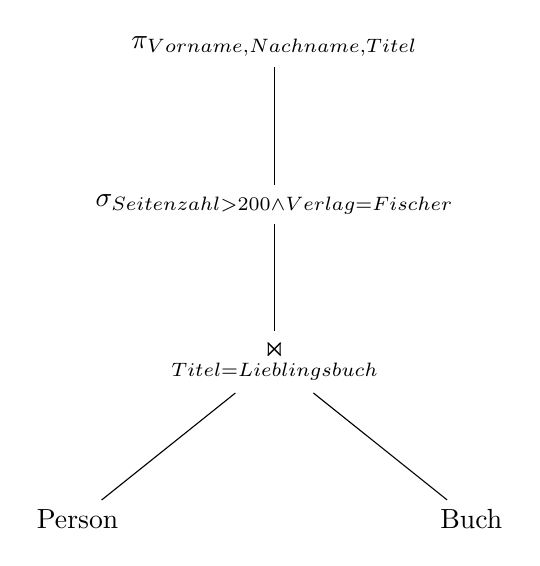
\begin{tikzpicture}
	\node (buch) at (2.5,0) {Buch}	
	node (person) at (-2.5,0) {Person}
	node (join1) at (0,2) {$\underset{Titel=Lieblingsbuch}{\Join}$}
	edge (person)
	edge (buch)
	node (selektion1) at (0,4) {$\sigma_{Seitenzahl>200\land Verlag=Fischer}$}
	edge (join1)
	node (projektion1) at (0,6) {$\pi_{Vorname,Nachname,Titel}$}
	edge(selektion1);
	
	\end{tikzpicture}
\end{center}
	
\subsection*{A3.}
\begin{center}
	\begin{tikzpicture}
	\node (buch) at (2.5,0) {Buch}
	node (selektion1) at (2.5,2) {$\sigma_{Seitenzahl>200}$}
	edge (buch)
	node (selektion2) at (2.5,4) {$\sigma_{ Verlag=Fischer}$}
	edge (selektion1)
	node (person) at (-2.5,4) {Person}
	node (join1) at (0,6) {$\underset{Titel=Lieblingsbuch}{\Join}$}
	edge (person)
	edge(selektion2)
	node (projektion1) at (0,8) {$\pi_{Vorname,Nachname,Titel}$}
	edge (join1);
	
	\end{tikzpicture}
\end{center}
Beim Vergleich von A1 und A3 stellt man fest, dass A1 einen höheren Optimierungsgrad hat als A3, da in letzterem zwei Selektionen hintereinander ausgeführt werden.\\
A1 hat auch einen höheren Optimierungsgrad als A2, denn die Join Operation wird hier vor der Selektion durchgeführt, was gemäß den Optimierungsheuristiken besagten Optimierungsgrad verringert.\\
A1 erreicht daher von allen gegebenen Ausdrücken den höchsten Optimierungsgrad. 
\end{document}
